\chapter{Revisión de Literatura}
\label{Capitulo_2}
\label{Literatura}
\section{Conexiones inalámbricas}
\subsection{Tipos de conexiones inalámbricas}

Además de la conectividad \acs{wifi}, existen otras tecnologías inalámbricas ampliamente utilizadas en dispositivos móviles, ordenadores personales y dispositivos \acl{iot}. Entre estas, \acl{ble} (\acs{ble}), una variante de Bluetooth diseñada para un consumo de energía extremadamente bajo, es especialmente relevante para aplicaciones \acl{iot} debido a su eficiencia energética y capacidad para operar en dispositivos alimentados por baterías durante largos períodos.

Otra tecnología inalámbrica importante es Zigbee, que utiliza el protocolo IEEE 802.15.4 para crear redes de área personal de baja potencia. Zigbee es común en aplicaciones de automatización del hogar y \acl{iot}, proporcionando una solución eficaz para controlar dispositivos inteligentes dentro de un hogar o edificio.

Las redes celulares, incluyendo tecnologías como 4G LTE y 5G, también juegan un papel crucial en la conectividad inalámbrica, ofreciendo cobertura a gran escala y soporte para una amplia gama de servicios móviles e \acs{iot}. Estas redes permiten la conectividad de dispositivos móviles y \acl{iot} en movimiento, soportando aplicaciones que requieren movilidad y acceso a internet de alta velocidad.

Finalmente, el \acl{lpwan} (\acs{lpwan}), incluyendo tecnologías como \acl{lora} y \acl{nbiot}, proporciona soluciones para aplicaciones \acl{iot} que requieren comunicaciones a larga distancia y bajo consumo de energía. Estas redes son ideales para sensores y dispositivos \acl{iot} distribuidos a lo largo de áreas extensas, como en aplicaciones de monitoreo ambiental y agricultura inteligente.

Se eligió utilizar \acs{wifi} como la tecnología para este sistema de seguimiento debido a varias razones prácticas. En primer lugar, la tecnología \acs{wifi} está presente en casi todos los teléfonos y muchos otros dispositivos, hasta incluso algunos autos. No hay necesidad de equipo extra o configuraciones especiales para detectar estos dispositivos, lo que lo hace muy accesible. Además, \acs{wifi} tiene un alcance más largo en comparación con tecnologías como Bluetooth, lo que permite cubrir áreas más grandes sin complicaciones. Otro punto a favor es que los dispositivos suelen buscar redes \acs{wifi} automáticamente, enviando solicitudes de sondeo de manera pasiva. Esto significa que se pueden rastrear sin que hagan algo activamente para ser detectados; esto convierte al \acs{wifi} en una tecnología ideal para monitorear movimientos y presencia en diversos entornos.

\subsection{Estados de conexión Wi-Fi}

Todos los dispositivos móviles, ordenadores personales y dispositivos \emph{IOT} que poseen conectividad Wi-Fi utilizan los mismos mecanismos de conexión. El esquema más común de topología de red es un \emph{Access Point} y múltiples dispositivos en modo cliente conectados a este. Por ejemplo, una laptop conectada a un router hogareño que le provee de internet.

\begin{figure}[!htb]
	\centering
	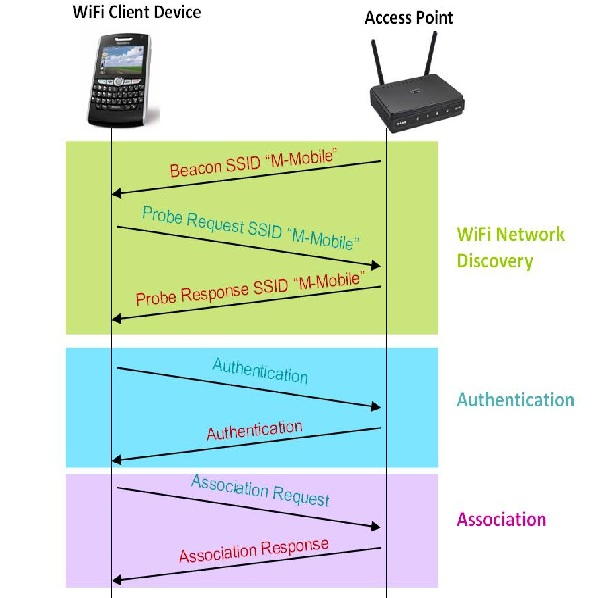
\includegraphics[width=0.6\textwidth]{Figuras/fig1.jpg}
	\captionsetup{margin=2cm}
	\caption[Secuencia de estado de la conexión]{Secuencia de estado de la conexión. Los paquetes de tipo Probe-Request o Beacon pertenecen a frames de clase 1. }
	\label{fig:frame-type}
\end{figure}

Si un dispositivo en modo cliente intenta conectarse a un \emph{Access Point} primero debe encontrarse en rango. Para saber que \emph{Access Points} están en rango para poder intentar la conexión, se utilizan dos paquetes que cumplen la misma función, pero lo realizan de maneras diferentes: Un paquete de tipo \emph{Probe Request} y un paquete \emph{Beacon}.

Un \emph{Beacon} es un tipo de paquete que emiten los \emph{Access Points} y tiene como objetivo anunciar a los clientes cercanos para que estos intenten conectarse si así lo desean. Un \emph{Probe Request} en cambio, es un paquete emitido por un cliente para solicitar información acerca de un \emph{Access Points} en particular o de todos los que se encuentren disponibles en un canal (banda inalámbrica para una frecuencia, ej., 2.4 GHz o 5 GHz).

Si un adaptador \acs{wifi} se encuentra en modo “promiscuo” o \emph{Sniffer}, podrá escuchar todos los paquetes y no solamente los que están dirigidos a dicho adaptador. Esto nos permitirá realizar una escucha pasiva, como mencionamos anteriormente. Por ende, un adaptador en dicho modo podrá recibir paquetes de todo tipo en particular, \emph{Probe-Request} de clientes y \emph{Beacon Frames}, de \emph{Access Points} respectivamente, que se encuentren en rango. 

Un cliente posee dos maneras de realizar un escaneo del área y determinar que \emph{Access Points} se encuentran presentes: un escaneo pasivo o un escaneo activo. 

Un escaneo pasivo (similar a un esquema de polling) consiste en sintonizar la antena de nuestro \emph{Sniffer} una fracción de tiempo a la vez en distintos canales (channel hopping). En cada canal se reciben \emph{Beacon Frames} pudiendo analizar así los \emph{Access Points} cercanos. 

Un escaneo activo, en cambio, envía \emph{Probe Request Frames} y espera \emph{Probe Response Frames} también usando opcionalmente \emph{Channel Hopping}. Esta estrategia es utilizada ampliamente por dispositivos móviles donde la batería es un factor a tener en cuenta y cuanto menos tiempo se necesite estar haciendo un escaneo, ya sea activo o pasivo, del área, mejor para el ahorro de energía del dispositivo en cuestión.

Entonces, de esta manera, un dispositivo podría activamente solicitar respuesta de un \emph{Access Point} en particular o de cualquiera en el área en vez de esperar a recibir un \emph{Beacon Frame}. Esto es beneficioso además, ya que asegura que ese \emph{Access Point} está en rango efectivo, ya que este pudo enviar su \emph{Probe Response} al cliente y este fue recibido exitosamente \cite{IEEE80211-2016}\cite{tanenbaum2011computer}.

\section{Técnicas de Posicionamiento}
\subsection{Intensidad de la Señal WiFi}

Para poder obtener la distancia a la que se encuentra un dispositivo inalámbrico, existen múltiples estrategias \cite{8692423} \cite{10.1007/1-4020-8155-3_8}. Una es enviar un mensaje (\emph{Ping}) y esperar la respuesta (\emph{Pong}). Con base en la diferencia entre el tiempo de emisión y el de respuesta, determinar la distancia según la velocidad de propagación de la onda electromagnética en el aire en promedio. Esta estrategia tiene el inconveniente de que sí requiere la cooperación del dispositivo del cual quiero obtener su posición, ya que necesito de su respuesta.

La otra alternativa es esperar a que el dispositivo inalámbrico cliente emita un paquete y medir su \acl{rssi} o \acs{rssi}. Este indicador representa una aproximación de la intensidad con la cual la antena inalámbrica receptora recibe el mensaje transmitido. Suele usarse a menudo en redes inalámbricas para determinar la calidad de la conexión entre dispositivos, pero puede aprovecharse para deducir su distancia (aplicando técnicas de predicción de la propagación del espectro electromagnético), como demuestra el estudio realizado por Barai et al. \cite{Barai2017EstimateDM}.

 Esta característica puede ser usada para, por ejemplo, visualizar la intensidad de la señal de los \emph{Access Point}\textit{s} que se encuentran en la cercanía, pero también sirve para que los \emph{Access Point}\textit{s} puedan saber la distancia a la que se encuentran sus clientes.

 

\subsection{Multilateración y Trilateración}

\begin{figure}[!htb]
	\centering
	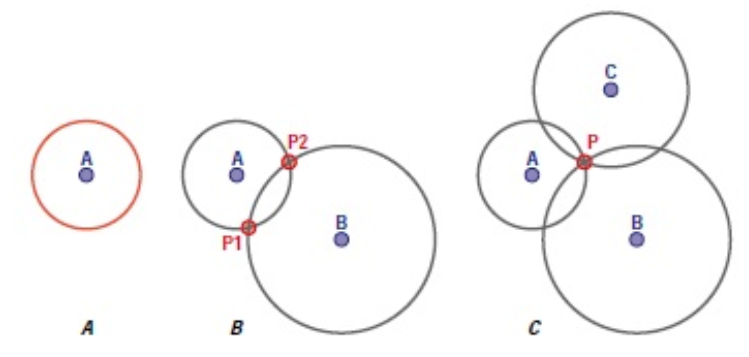
\includegraphics[width=0.7\textwidth]{Figuras/fig4.png}
	\captionsetup{margin=2cm}
	\caption[Casos Trilateración]{ Tipos de intersecciones. Utilizando el método clásico de trilateración, se pueden observar por lo menos tres casos.}
	\label{fig:tri}
\end{figure}

 Utilizando un \emph{Sniffer} para recibir los paquetes de tipo \acl{prq} o \emph{Beacon Frame} que se encuentran en un área y obteniendo el \acs{rssi} de cada paquete, es posible estimar la distancia a la que se encuentra un objetivo desde nuestro \emph{Sniffer} (caso A). Sin embargo, si se tiene más de un \emph{Sniffer} (B y C) y de cada uno conozco su ubicación precisa, puede entonces estimar la posición geográfica del cliente mediante multilateración.

La trilateración y la multilateración son técnicas matemáticas que se utilizan para determinar las coordenadas desconocidas de un punto en el espacio, basándose en las distancias desde ese punto a varios puntos conocidos. En el caso del GPS, un receptor mide la diferencia en el tiempo de llegada de las señales de al menos cuatro satélites, lo que permite calcular su posición tridimensional (latitud, longitud y altitud). De manera similar, en un entorno de localización basado en \acs{wifi}, los puntos conocidos serían los sensores \acs{wifi} que registran la presencia de otros dispositivos, y la ubicación desconocida sería la del dispositivo objetivo \cite{bulusu2000gps}.

La figura \ref{fig:tri} ilustra el concepto de trilateración, que es la base para entender la multilateración. En un contexto ideal, con tres círculos que se intersectan en un único punto, se puede determinar la ubicación exacta del dispositivo. Sin embargo, en la práctica, debido a factores como la interferencia de señales, los reflejos y la atenuación, las estimaciones de distancia basadas en \acs{rssi} pueden no ser precisas \cite{rappaport2002wireless}, lo que lleva a la necesidad de utilizar múltiples mediciones y aplicar técnicas de optimización para encontrar la mejor estimación de la posición\cite{ouyang2010received}\cite{li2012kalman}.

La multilateración es un proceso avanzado de localización que extiende los principios de la trilateración para estimar la posición de un objeto en dos o tres dimensiones. Mientras que la trilateración se basa en las distancias medidas desde tres puntos conocidos (en 2D) o cuatro puntos (en 3D) hasta el punto de interés, la multilateración utiliza señales de cuatro o más puntos para realizar la estimación, lo que mejora significativamente la precisión y la fiabilidad de la localización, especialmente en entornos complejos.

El proceso de multilateración implica la resolución de un sistema de ecuaciones que representan las distancias estimadas desde los nodos conocidos hasta el dispositivo. Este sistema puede ser linealizado y resuelto mediante el método de los cuadrados mínimos, como veremos más adelante en la sección \ref{sec:lsq}, para encontrar la ubicación que mejor se ajuste a las mediciones observadas. 

Entonces, hasta ahora podemos identificar a un dispositivo en particular y si se encuentra en rango de al menos uno de nuestros sensores que 

A partir de ahora llamaremos \emph{Sniffers} y sabremos su ubicación con mayor o menor precisión según cuantos \emph{Sniffers} tengamos en el área. Para poder seguir efectivamente la trayectoria de un individuo, es necesario poder identificar inequívocamente al dispositivo que se quiere rastrear a lo largo del tiempo. Esto es posible ya que cada paquete \emph{Probe Request} y \emph{Beacon Frame} contiene la \textit{\acs{mac} Address} del dispositivo que sirve como identificador único. 

\subsection{ Aleatorización de MAC Addresses}

Existen dispositivos que implementan técnicas de randomización de direcciones \acs{mac} \cite{martin2017study}; en este caso, se asigna periódicamente una dirección \acs{mac} aleatoria como medida de protección de la privacidad. Esta práctica complica el seguimiento continuo de dichos dispositivos y dificulta la estimación precisa del número de dispositivos presentes en una determinada área, puesto que el mismo dispositivo podría ser contabilizado en varias ocasiones bajo distintas direcciones \acs{mac}.

 Sin embargo, esta técnica no es aún ampliamente usada al momento de escribir este trabajo [1] e incluso se cuenta con la posibilidad de distinguir rápidamente si una \textit{\acs{mac} Address} es local (randomizada) o global (no randomizada) pudiendo así descartar “el ruido”.

Además, los dispositivos móviles \cite{freudiger2015talkative} suelen emitir los paquetes \acl{prq} en grandes ráfagas sin cambiar la \textit{\acs{mac} Address} incluso cuando estos tienen activada la randomización. Esto implica que, si bien no es posible saber en principio si es el mismo dispositivo el que desapareció de la ubicación anterior y luego reapareció en una nueva, al tener más de un \acl{prq} puedo saber su velocidad y dirección.

Lo que es más, sabiendo estos dos datos, es posible predecir que dos \textit{\acs{mac} Address} son distintas (randomizadas) sean en verdad pertenecientes al mismo dispositivo.

No obstante, aunque el dispositivo no randomice, es necesario para poder saber el recorrido completo de un dispositivo en un área, haciendo necesario algún tipo de algoritmo de predicción de desplazamiento. Ya que a no ser que todos los \emph{Sniffer}\textit{s} cubran el área en cuestión de manera completa, y no haya ninguna anomalía en la recepción. Van a haber secciones del recorrido que no van a poder ser capturadas por los \emph{Sniffer} ya sea por un problema de rango, de espacios ciegos, o bien porque el dispositivo cliente no emite la suficiente cantidad de \acl{prq} como para poder hacer un seguimiento más exhaustivo. Esto sin mencionar las anomalías de mediciones, ya sea por interferencia o por paredes en el medio que bajan la señal recibida a pesar de que el dispositivo no esté más lejos. 

En este trabajo, sin embargo, no exploramos el problema de la randomización ni el problema de los espacios ciegos. Nos limitaremos a ubicar en el espacio y el tiempo a un dispositivo en modo \emph{Access Point} emitiendo paquetes \emph{Beacon Frame}. De esta manera nos aislamos del problema de la randomización, además de tener una buena frecuencia regular de datos sin interrupciones, que es fundamental para los experimentos realizados.

\section{Medición de distancia en base al modelo de \textit{Path Loss}}

Para poder realizar el paso de multilateración, primero es necesario conocer la distancia desde cada uno de los \emph{Sniffer} hacia el \emph{“Objetivo”}. Para ello se usará en este trabajo la medición de \acs{rssi} y luego, para convertir de \acs{rssi} a distancia, basándonos en trabajos previos \cite{doi:10.4236/wsn.2010.28072} \cite{doi:10.1155/2014/371350}, se decidió usar un modelo derivado de la fórmula de pérdida en el trayecto de propagación o \emph{Path Loss}. Mediante el cual la pérdida de señal se incrementa proporcionalmente al logaritmo de la distancia recorrida.

Este modelo describe cómo la intensidad de una señal electromagnética disminuye a medida que se propaga a través del espacio. La pérdida ocurre debido a diversos factores como la dispersión, absorción y difracción de la señal, y se incrementa proporcionalmente a la distancia recorrida desde la fuente emisora. Esta atenuación de la señal es esencialmente una consecuencia de la expansión de las ondas electromagnéticas en el espacio, lo que resulta en una reducción de la densidad de potencia a medida que la distancia aumenta.

\newline
\newline

La fórmula general de \emph{Path Loss} en el espacio libre se puede expresar como:

\begin{equation}
    P(d)=P(d_{0}) - 10n*log(\frac{d}{d_{0}}) - X_{\sigma}
\end{equation}
Donde:
\begin{conditions}
 d         &  distancia (m)\\
 d_{0}   &  distancia de referencia inicial (m) \\
P(d)        &  es la potencia recibida en la distancia d \\
P(d_{0})   &  potencia en la distancia de referencia inicial (\acs{dbm}) \\
X_{\sigma} &  es una variable de ajuste que está relacionada directamente con la incertidumbre del modelo.\\
\end{conditions}
Luego podemos asumir que la distancia de referencia será 1 metro y agregar una variable A’ que ajustaremos para calibrar nuestra fórmula, reemplazando a \(P(d_{0})\) y \(X_{\sigma}\).
\begin{equation}
    RSSI = A' -10n*log(d)
\end{equation}
Finalmente, podemos simplificar aún más dividiendo por 10 y reemplazando \(A'/10\) por \(A\)
\begin{equation}
    RSSI = A - n*log(d)
\end{equation}

Ahora sólo resta hallar el valor de A y N para nuestros 

\emph{Sniffers} en el ambiente donde deseamos realizar la medición. Sin embargo, debido a las interferencias que ya mencionamos, en algunos escenarios puede ser necesario algún proceso que permita filtrar la señal para luego después proceder a hacer el siguiente paso de ajuste logarítmico.

\section{Ajuste Logarítmico}

El ajuste logarítmico juega un papel crucial en la modelización de la relación entre la intensidad de la señal recibida (\acs{rssi}) y la distancia en aplicaciones de localización y seguimiento. Este proceso implica ajustar un modelo matemático que mejor se acomode a los datos observados, permitiendo así predecir la distancia a partir de los valores de \acs{rssi}.

\lstset{style=codestyle}
\begin{figure}[!htb]
\centering
\begin{lstlisting}[language=Python]
def fit_parameters(distance, signal, A=0, N=0):
    """
    Ajusta los parámetros del modelo logarítmico para estimar la relación entre
    la distancia y el RSSI.
    distance (list): Lista de distancias medidas.
    signal (list): Lista de valores de señal RSSI correspondientes a las distancias.
    A (float): Valor inicial de A (por defecto 0).
    N (float): Valor inicial de N (por defecto 0).
    
    Retorna:
    tuple: Valores ajustados de A y N, y la métrica de calidad del ajuste.

    """
    # Define una estimación inicial para a y n.
    initial_guess = dict(a=A, n=N)
    # Crear un modelo utilizando la función distance_to_rssi
    regressor = lmfit.Model(distance_to_rssi)
    # Ajustar el modelo a los datos usando el método de Cuadrados Mínimos Secuenciales (SLSQP)
    results = regressor.fit(signal, d=np.array(distance), **initial_guess, method="slsqp")
    # Calcular el residual como la norma de la diferencia entre la señal observada y la predicha.
    residual = np.linalg.norm(signal - distance_to_rssi(distance,
                                                     results.values['a'],
                                                    results.values['n']))

    # Retornar los parámetros ajustados y la métrica de calidad del ajuste (100 - residual)
    return results.values['a'], results.values['n'], 100 - residual

def distance_to_rssi(d, a, n):

    """
    Modelo que describe la relación entre la distancia y el RSSI.
    d (float): Distancia entre el emisor y el receptor.
    a (float): Parámetro A del modelo.
    n (float): Parámetro N del modelo.
    Retorna:
    float: Valor de RSSI correspondiente a la distancia d.

    """
    # Ecuacion del modelo para convertir la distancia en RSSI

    return - (n * np.log10(d) + a)

def rssi_to_distance(rssi_values, a, n):

    """
    Convierte valores de RSSI a estimaciones de distancia utilizando el modelo ajustado.
    Retorna:
    list: Lista de distancias estimadas correspondientes a los valores de RSSI.
    """
    distances = []
    for rssi in rssi_values:
        # Usar la inversa de la ecuación distance_to_rssi para encontrar la distancia
        distances.append(10 ** (-1 * (rssi + a) / n))
    return distances

\end{lstlisting}
\caption{Script Python para ajuste de curva. Código disponible en 
\label{fig:log-fit-script}
\href{https://github.com/agusalex/rssi-filter-profiling/blob/wip/profiler.py}{GitHub}.  }
\end{figure}

Para llevar a cabo el ajuste logarítmico, se empleó la biblioteca \textbf{lmfit} en \textit{Python}, la cual ofrece herramientas avanzadas para la optimización y solución de ecuaciones lineales y no lineales. En particular, se utilizó el método de \textit{Cuadrados mínimos Secuenciales} (\acs{slsqp}), que permite encontrar los valores óptimos de los parámetros del modelo que minimizan la diferencia entre los valores predichos por el modelo y los observados en la realidad.

El proceso de ajuste comenzó con la selección de una función a la que ajustar, en este caso, la función logarítmica ya mencionada que describe cómo el \acs{rssi} varía con la distancia. Basada en la teoría de pérdida de trayectoria (\textit{Path Loss}).

El ajuste del modelo se realizó sobre un conjunto de datos que consiste en mediciones de \acs{rssi} y las correspondientes distancias reales, utilizando como valores iniciales una aproximación de los parámetros \textbf{A} y \textbf{N}, que representan la intensidad de señal a una distancia de referencia y el decaimiento de la señal con la distancia, respectivamente.

\subsection{Modelo Matemático}
\begin{figure}[!htb]
	\centering
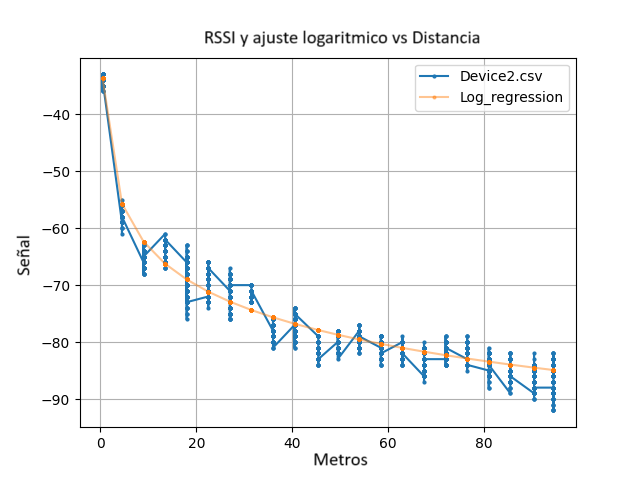
\includegraphics[width=0.8\textwidth]{Figuras/profiling/device2/device2-profiling.png}
	\captionsetup{margin=2cm}
	\caption[\acs{rssi} segregado por distancia de la medición vs regresión logarítmica, prueba de campo]{\acs{rssi} segregado por distancia de la medición vs regresión logarítmica, prueba de campo, con \acs{esp} en campo de deportes \acs{ungs}}.
	\label{fig:log-fit}
\end{figure}

La relación entre \acs{rssi} y la distancia se modela con la misma ecuación ya mencionada en la sección anterior. Con una pequeña diferencia en los signos para obtener números positivos.

\begin{equation}
    \text{RSSI} = -A - N \cdot \log(d)
\end{equation}

donde:

\begin{itemize}
    \item \(d\) representa la distancia entre el dispositivo emisor y el receptor.
    \item \(A\) es el valor de \acs{rssi} medido a una distancia de referencia de 1 metro. Que en vez de averiguar de manera experimental, procedemos a calcularlo usando las técnicas mencionadas.
    \item \(N\) es el coeficiente de pérdida de trayectoria, que refleja cómo la señal se atenúa con el incremento de la distancia.
\end{itemize}

Esta fórmula ajusta el \acs{rssi} observado a un modelo logarítmico, donde \(a\) y \(n\) son parámetros clave que se optimizan para ajustar el modelo a los datos recogidos.

Para convertir los valores de \acs{rssi} en estimaciones de distancia, se utiliza la inversión de la fórmula anterior:

\begin{equation}
    d = 10^{(-1 \cdot (\text{RSSI} + a) / n)}
\end{equation}

Para evaluar la bondad del ajuste, se calculó el residual como la norma euclidiana de la diferencia entre los valores observados y los predichos por el modelo. Este residual proporciona una medida cuantitativa de la discrepancia entre el modelo y los datos reales, sirviendo como indicador de la precisión del ajuste.

\begin{equation}
    \text{residual} = \lVert \text{RSSI observado} - \text{RSSI predicho} \rVert
\end{equation}

El valor de R, definido como $100 - \text{residual}$, ofrece un indicador para interpretar la calidad del ajuste; valores cercanos a 100 indican un ajuste muy preciso, mientras que valores más bajos sugieren una mayor discrepancia entre el modelo y los datos reales.

\subsection{Implementación}

Se implementaron scripts en \textit{Python} para realizar el ajuste logarítmico y el cálculo del residual, como el extracto que se puede ver en \ref{fig:log-fit-script} y cuyo código completo se encuentra en la sección \ref{herramientas_software}. Estos scripts permiten automatizar el proceso de ajuste y evaluación para diferentes conjuntos de datos, facilitando la experimentación y el análisis.

La figura \ref{fig:log-fit} muestra un ejemplo de gráfica resultante de aplicar dicho script, ilustrando cómo el modelo ajustado se alinea con las mediciones reales de \acs{rssi} segregadas por distancia.

\section{Filtrado de Kalman}
\begin{figure}[!htb]
	\centering
	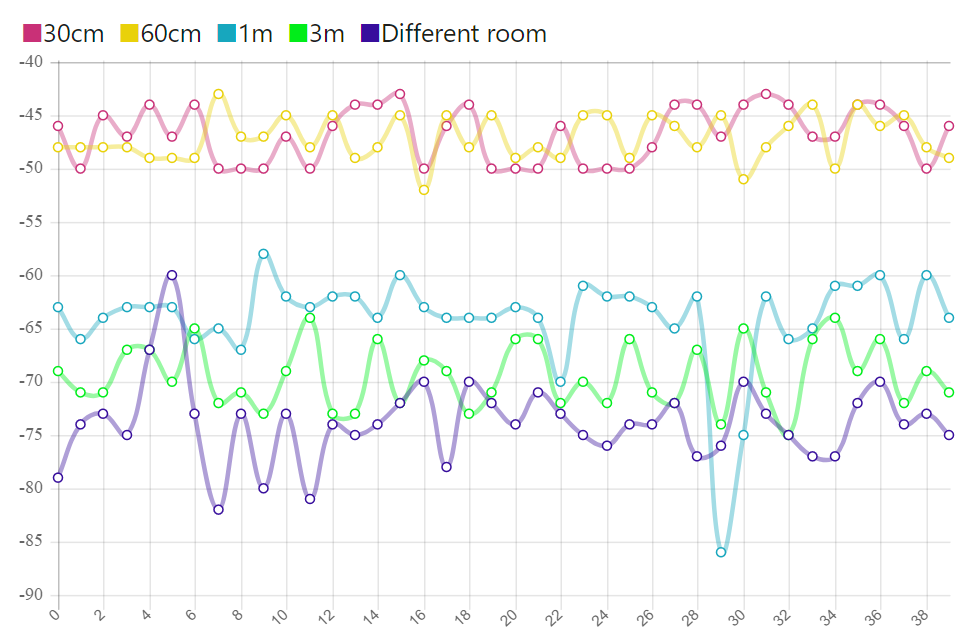
\includegraphics[width=0.8\textwidth]{Figuras/fig6.png}
	\captionsetup{margin=2cm}
	\caption[\acs{rssi} recibido a distintas distancias]{\acs{rssi} recibido a distintas distancias. (Kalman filters explained: Removing noise from \acs{rssi} signals. Wouter Bulten)}
	\label{fig:rssi-wouter}
\end{figure}

\begin{figure}[!htb]
	\centering
	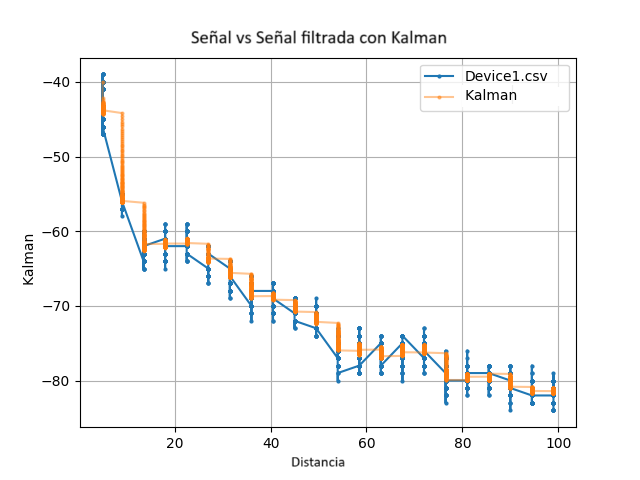
\includegraphics[width=0.8\textwidth]{Figuras/profiling/device1/Device1Kalman.png}
	\captionsetup{margin=2cm}
	\caption[Medicion de \acs{rssi} original y filtrada con Kalman, prueba de campo con \acs{esp} en campo de deportes \acs{ungs}]{Medicion de \acs{rssi} original y filtrada con Kalman, prueba de campo con \acs{esp} en campo de deportes \acs{ungs}}
	\label{fig:filtrado-kalman}
\end{figure}

El filtro Kalman es un algoritmo recursivo muy versátil que se utilizó en este trabajo  para estimar con más precisión la distancia a partir del \acs{rssi} recibido. Sobre todo en presencia de ruido e interferencia. Se decidió utilizar dicho filtro basándonos en el trabajo de Wouter Bulten et al. \cite{7471364} y del cual deriva un script en Python adaptado del original en Javascript por Sifan Ye \cite{SifanYe}. También se consultó como referencia otros trabajos similares como el de Tsanousa et al. \cite{tsanousa2021localization}.

Dicho filtro consiste en un estimador de estado que realiza una estimación de alguna variable no observada (en nuestro caso el \acs{rssi} real derivado de las mediciones observadas) basándose en mediciones ruidosas y teniendo en cuenta el historial de las mediciones anteriores. Un filtro de Kalman tradicional asume modelos lineales. Es decir, el paso del estado actual al siguiente debe ser una transformación lineal.

Se usará la identidad como matriz de transformación \(At\), y como no hay control sobre el movimiento, la matriz de control \(Bt\) se asume nula. Lo mismo ocurre con \(Vt\) el cual dejaremos en 0, ya que inicialmente asumiremos que no hay control sobre el objetivo. Finalmente, como el estado es modelado directamente, la matriz de observación \(Ct\) también se igualará a la identidad. Por otro lado, \(\epsilon_{t}\) y \(\theta_{t}\) representan el ruido de proceso y de medición, respectivamente.

 En consecuencia, el modelo de transición y observación se puede representar de la siguiente manera:

\[X_{t} = A_{t} * X_{t-1} + B_{t} + V_{t} + \epsilon_{t} = X_{t-1} + \epsilon_{t} \]

El paso predictivo lo calcularemos de la siguiente manera, donde R es el ruido de proceso que provendría del sistema en sí. Como sabemos que en este caso el ruido proviene de la medición y no del sistema, se asume un valor bajo (0.008). \(\sum\) se puede utilizar como indicador de la certeza de nuestra predicción. Entonces nos queda que la certeza en el paso \(t\) es igual a la certeza en el paso anterior más el ruido de proceso actual definido con la siguiente fórmula:

\[ \mu_{t}' = \mu_{t-1}  \]

\(\mu\) describe la predicción y x es el verdadero valor del estado. \(\mu’\) a diferencia de \(\mu\) indica que todavía no hemos incorporado la información sobre la medición. Es decir, es una predicción tentativa. Lo mismo aplica con Z y Z’.
\[\sum t' = \sum (t-1)' + R_{t} \]

La ganancia de Kalman, sera nuestra función de ponderación. Para ello usaremos Q como el ruido de medición; este indicador de ruido es más importante para este caso y deberá ser ajustado si se sabe que la interferencia puede deberse al movimiento del objetivo. Sin embargo, como inicialmente asumimos un modelo estático, entonces Q=3. La fórmula de la ganancia de Kalman entonces será la siguiente: 

\[K_{t} = K_{t}' ( \sum t' + Q_{t})^-1\]

Finalmente, el paso de actualización será de la siguiente manera:

\[ \mu_{t} = \mu_{t}' + K_{t}(Z_{t}-\mu_{t}')\]
\[ \sum t = \sum t' - (K_{t} \sum t')\]

En este último paso podemos notar que estamos calculando \(\mu_{t}’\), o sea la predicción final del sistema. Además, también hallamos el valor de \(\sum t\), nuestra certeza de predicción.
Este filtro logra adaptarse al entorno, decidiendo en base al histórico cuánta importancia darle a las nuevas mediciones por sobre las anteriores, ignorando el ruido a medida que este se agranda.

%\begin{figure}[th]

%	\centering

	%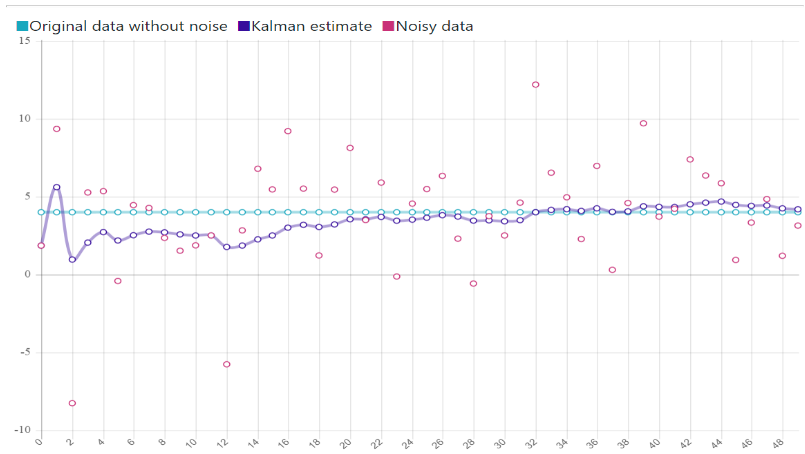
\includegraphics[width=0.8\textwidth]{Figuras/fig7.png}

%	\captionsetup{margin=2cm}

%	\caption[Datos con ruido vs kalman filter vs Datos verdaderos]{Datos con ruido vs Estimativo Kalman vs Datos originales. (Lightweight Javascript library for Noise filtering using Kalman filters)}

%	\label{fig:rssi-wouter-2}

%\end{figure}

Sin embargo, como este sistema no tiene manera de saber si el ruido de medición Q es producto del ambiente o producto de movimiento orgánico del objetivo, se podrá modificar luego el valor de \(V_{t}\) y \(B_{t}\) para indicar movimiento cuando lo haya y dejar de asumir así que se trata de un sistema estático. Se explorará esto más adelante en la sección de Multilateración.

En este trabajo usaremos las técnicas de filtrado \textit{Kalman} como paso previo de procesamiento antes de utilizar las capturas obtenidas por los nodos. De esta manera eliminamos gran parte de la interferencia momentánea o errores de medición y le damos más foco a la trayectoria de la señal en vez de los accidentes temporales que producen su fluctuación.

\section{Cuadrados Mínimos aplicado a Multilateración}

\label{sec:lsq}

Para resolver el problema de ubicar en 2D al objetivo solo teniendo las distancias estimadas hacia cada uno de los \textbf{Sniffers} es necesario algún algoritmo de localización. En este caso, como no se tiene el dato de la dirección en la que viene la señal, una triangulación no es posible. Para ello se usará en este trabajo el método de trilateración, cuya versión extendida a n nodos se llama multilateración, mediante el método de \textbf{Cuadrados mínimos}. Se evaluó durante el desarrollo de este trabajo la posibilidad de usar filtros de partículas como método de localización; sin embargo, dada su complejidad, queda para trabajo futuro analizar qué impacto de performance y precisión podría tener sobre experimentos simulados y reales.

La ecuación objetivo a resolver se plantea de la siguiente manera:

\begin{equation}
(x - x_0)^2 + (y - y_0)^2 = (dist_0 - r )^2
\end{equation}
\begin{equation}
\ldots
\end{equation}
\begin{equation}
(x - x_n)^2 + (y - y_n)^2 = (dist_n - r )^2
\end{equation}

Donde \textbf{Y}, \textbf{X} y \textbf{R} son las incógnitas a resolver, \textbf{Xi} e \textbf{Yi} son la posición del \textit{Sniffer} que capturó la señal, \textbf{dist\_i} es la distancia predecida en base al \acs{rssi} capturado, aplicando nuestra fórmula de Path Loss con el \textbf{A} y \textbf{N} hallados anteriormente. Se asume los mismos \textbf{A} y \textbf{N} para cada nodo; sin embargo, existen trabajos donde, durante la etapa \textit{offline}, es decir, cuando se calibra la señal, se usa un \textbf{A} y un \textbf{N} distinto por cada nodo e incluso uno distinto por cada orientación de nodo \cite{etter2019simulation}. A pesar de esto, se decidió optar por un modelo más simple, ya que en simulaciones dio buenos resultados.